\documentclass[11pt]{article}
\usepackage{amsmath,amsthm,amsfonts,amssymb,amscd}
\usepackage{multirow,booktabs}
\usepackage[table]{xcolor}
\usepackage{fullpage}
\usepackage{lastpage}
\usepackage{enumitem}
\usepackage{fancyhdr}
\usepackage{mathrsfs}
\usepackage{wrapfig}
\usepackage{setspace}
\usepackage{calc}
\usepackage{multicol}
\usepackage{cancel}
\usepackage[retainorgcmds]{IEEEtrantools}
\usepackage[margin=3cm]{geometry}
\usepackage{amsmath}
\newlength{\tabcont}
\setlength{\parindent}{0.0in}
\setlength{\parskip}{0.05in}
\usepackage{empheq}
\usepackage{framed}
\usepackage[most]{tcolorbox}
\usepackage{xcolor}
\colorlet{shadecolor}{orange!15}
\parindent 0in
\parskip 12pt
\geometry{margin=1in, headsep=0.25in}
\theoremstyle{definition}
\newtheorem{defn}{Definition}
\newtheorem{reg}{Rule}
\newtheorem{exer}{Exercise}
\newtheorem{note}{Note}

\usepackage{pgfplots}
\usepackage{tikz}
\usetikzlibrary{3d} % TikZ 3D library for real 3D support
\pgfplotsset{compat=1.18} % Ensure compatibility with your LaTeX distribution



\begin{document}

% the counter below determines the sections and chapters:
\setcounter{section}{0}

\title{Robotic Principles Notes}

\thispagestyle{empty}

\begin{center}
{\LARGE \bf Robotic Principles Notes}\\
{\large 5ELEN018W.1}\\
SEM1 2024
\end{center}

% Part 1: Lectures 1 to 6 (FOR NOW)
\section{Spatial Descriptions and Transformation Matrices for Robotic Manipulators}
\subsection{Position Vector}
Spatial descriptions for Robotic Manipulators will help us calculate Velocities, Forces, and Torques.

\begin{note}
\textbf{The first step in finding the whereabouts of any robotic manipulator is to describe its position in 3D space.}
\end{note}

Any position or point is given with respect to a coordinate system. 

\begin{figure}[h]
    \centering
    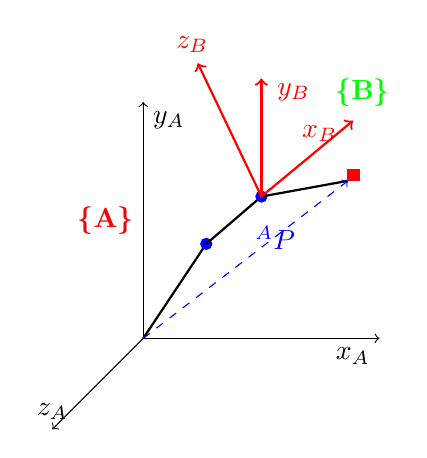
\begin{tikzpicture}
        % Draw the x-axis
        \draw[->] (0,0,0) -- (3,0,0) node[anchor=north east] {$x_A$};
        % Draw the y-axis
        \draw[->] (0,0,0) -- (0,3,0) node[anchor=north west] {$y_A$};
        % Draw the z-axis
        \draw[->] (0,0,0) -- (0,0,3) node[anchor=south] {$z_A$};

        % Draw the robot arm
        \draw[thick] (0,0,0) -- (0.8,1.2,0) coordinate (joint1);  % First link to joint
        \filldraw [blue] (joint1) circle (2pt);               % First joint

        \draw[thick] (joint1) -- (1.5,1.8,0) coordinate (joint2); % Second link to joint
        \filldraw [blue] (joint2) circle (2pt);                  % Second joint

        \draw[thick] (joint2) -- (2.6,2,0) coordinate (endEffector); % End effector link
        \filldraw [red] (endEffector) rectangle +(4pt,4pt);                  % End effector
        % Add label {A} close to the left of the y-axis
        \node[left, red] at (0, 1.5, 0) {\textbf{\{A\}}};
        
        %Draw an arrow from origin to the end effector and label it A_p
        \draw[->, dashed, blue] (0,0,0) -- (endEffector) node[midway, above right] {\textbf{${}^{A}P $}};    
        
        % Draw enlarged red x, y, z axes at the second joint
        \draw[->, red, thick] (joint2) -- ++(0.2,0,-2.5) node[anchor=north east, xshift=-2pt, yshift=2pt] {\textbf{$x_B$}};
        \draw[->, red, thick] (joint2) -- ++(0,1.5,0) node[anchor=north west, xshift=2pt, yshift=2pt] {\textbf{$y_B$}};
        \draw[->, red, thick] (joint2) -- ++(-1,1.5,-0.5) node[anchor=south, xshift=-2pt] {\textbf{$z_B$}};   
        
        % Add label {B} in green close to the new coordinate set
        \node[right, green] at (2.7, 3.5, 1) {\textbf{\{B\}}};
        
    \end{tikzpicture}
    \caption{3D Simple Robot Arm}
\end{figure}
In Figure 1,we can see the \textit{Frame A}, or coordinate system.
The position of any links or he \textit{End Effector} is given using a position vector, denoted by ${}^{A}P $.

\begin{equation}
    {}^{A}P = \begin{bmatrix} x_{A} \\ y_{A} \\ z_{A} \end{bmatrix}
\end{equation}

$A$ represents the Coordinate System, whilst $P$ is the Position Vector.
If Cartesian coordinates are used the position of a point in space can be given by its $x$, $y$, $z$ components.

\subsection{Orientation Matrix}
Along with the position, the orientation of the manipulator must also be described. This shows how it is angled or oriented in space. \\
Here a Coordinate Frame '$B$' has been assigned, showing how the $x$, $y$, $z$ axis are set for this particular part of the robot.\\
Using this, the orientation of $B$ can be expressed relative to any previous coordinate frame, in this case, $A$.

Numerically the orientation is expressed using a three by three rotation matrix, which comprises of a stack of the unit vectors in the $x$, $y$, $z$ directions going from $B$ to $A$:
\begin{equation}
{}^{A}_{B}R = \begin{bmatrix} {}^{A}\hat{X}_{B} \quad {}^{A}\hat{Y}_{B} \quad {}^{A}\hat{Z}_{B} \end{bmatrix} = \begin{bmatrix} r_{11} \quad r_{12} \quad r_{13} \\ r_{21} \quad r_{22} \quad r_{23} \\ r_{31} \quad r_{32} \quad r_{33} \end{bmatrix}
\end{equation}

The notation ${}^{A}_{B}R$ shows the orientation of $B$ relative to $A$. 

\subsection{Frames}
By combining the orientation matrix and position vector we can now fully describe the whereabouts of any robotic manipulator. This is known as a \textit{Frame}. Note that the Frame is just another coordinate system where the position of its origin, in this case $B$-origin and its orientation are known with respect to a previous coordinate system, in this case $A$.
\begin{shaded}
\begin{equation}
\{B\} = \{{}^{A}_{B}R, {}^{A}P_{Borg}\}
\end{equation}
\end{shaded}

% ---------------- TBC !!!!

\subsection*{Addition of Angular Velocities}
One can add angular velocities just like linear velocities. If body 3 is rotating at angular velocity $\omega_{32}$ relative to frame 2, and frame 2 is rotating at angular velocity $\omega_{21}$ relative to frame 1, then body 3 is rotating relative to frame 1 at angular velocity: 
\begin{equation}
\omega_{31} = \omega_{32} + \omega_{21}
\end{equation}
\subsection{Time Derivatives in Rotating Frames}
If frame S has a angular velocity, $\Omega$ relative to S$_0$ then the time derivative of a single vector \textbf{Q} as seen in the two frames are related by:
\begin{equation}
(\frac{d\textbf{Q}}{dt})_{S_0} = (\frac{d\textbf{Q}}{dt})_{S} \ + \Omega \ x \ \textbf{Q}
\end{equation}
\subsection{Netwon's Second Law in a Rotating Frame}
A particle in an inertial reference frame, S$_0$ obeys Newton's second law as we are use to:
\begin{equation}
m\frac{d^2r}{dt^2} = F
\end{equation}
Using the results from equation 8, the time derivative for a rotating frame with reference to an inertial frame can be given by:
\begin{equation}
(\frac{dr}{dt})_{S_0} = (\frac{dr}{dt})_s \ + \Omega \ x \ r
\end{equation}
By differentiation, Newton's second law becomes:
\begin{equation}
m\ddot{r} = F + 2m\dot{r} \ x \ \Omega \ + m(\Omega \ x \ r) \ x \ \Omega
\end{equation}
Where \textit{F} is the sum of all forces in the inertial reference frame. 
\subsection{The Centrifugal Force}
This is an inertial force in a rotating reference frame 
\begin{equation}
F_{\text{cf}} = m(\Omega \ x \ r) \ x \ \Omega
\end{equation}
\subsubsection*{Free-Fall Acceleration (Non-Vertical Gravity)}
\begin{equation}
F_{\text{eff}} = F_{\text{grav}} + F_{\text{cf}} = mg_0 + m\Omega^2R\sin(\theta)\hat{\rho}
\end{equation}
The acceleration due to the Centrifugal force is simply 
\begin{equation}
\begin{split}
g = g_0 + \Omega^2R\sin(\theta)\hat{\rho} \\
g_{\text{rad}} = g_0 - \Omega^2R\sin^2(\theta)  \\
g_{\text{tan}} = \Omega^2R\sin(\theta)\cos(\theta)
\end{split}
\end{equation}
The angle between g and its radial direction is:
\begin{equation}
\alpha \approx \frac{g_{\text{tan}}}{g_{\text{rad}}} 
\end{equation}
The maxium value at ($\theta$ = 45):
\begin{equation}
\alpha_{\text{max}} =  \frac{\Omega^2R}{2g_0}
\end{equation}
\subsection{Coriolis Force}
The Coriolis Force is another inertial force in a rotating reference frame that an object experiences when it is moving. 
\begin{equation}
F_{\text{cor}} = 2m\dot{r} \ x \ \Omega = 2mv \ x \ \Omega
\end{equation}
The maximum acceleration, \textit{a} that the Coriolis force could produce acting by itself with \textit{v} perpendicular to $\Omega$ is:
\begin{equation}
a_{\text{max}} = 2v\Omega 
\end{equation}
\begin{shaded}
\textbf{Direction of the Coriolis Force} \newline
The Direction of the Coriolis force us always perpendicular to the velocity of the object (hence equation 17), and is given by the right hand rule. 
\end{shaded}
\newpage
\subsection{Free Fall and the Coriolis Force}
\begin{equation}
m\ddot{r} = mg_0 + F_{\text{cf}} + F_{\text{cor}} 
\end{equation}
\subsection{The Foucault Pendulum}
See chapter 9, Page 354. There is no need to recopy what is in the book here. 

\end{document}
